%%%%%%%%%%%%%%%%%%%%%%%%%%%%%%%%%%%%%%%%%%%%%%%%%%%%%%%%%%%%%%%%%
% > METODOS TRADICIONAIS DE INTEGRACAO NUMERICA
%%%%%%%%%%%%%%%%%%%%%%%%%%%%%%%%%%%%%%%%%%%%%%%%%%%%%%%%%%%%%%%%%
\section{Métodos tradicionais de integração numérica}
\subsection{Integradores básicos de primeira ordem}

Considere o problema \ref{eq:problema_de_cauchy}. Uma primeira ideia para produzir métodos numéricos é utilizar da linearização fornecida pela primeira derivada temporal para, a partir de um instante $t_k$, aproximar a trajetória no instante $t_{k+1}$, o que naturalmente é possível para qualquer problema de Cauchy bem posto. Essa aproximação é chamada de \textit{método de Euler explícito}.

\begin{method}[Euler explícito]\label{metodo:euler_explicito}
    Para $h=(b-a)/m$ e $k = 0, 1, ..., m-1$, temos a aproximação:
    \begin{equation*}
        t_{k+1} = t_k + h, \quad
        y_{k+1} = y_k + h f (t_k, y_k) = \Phi_h(t_k, y_k).
    \end{equation*}
\end{method}

\begin{figure}[H]
    \centering
    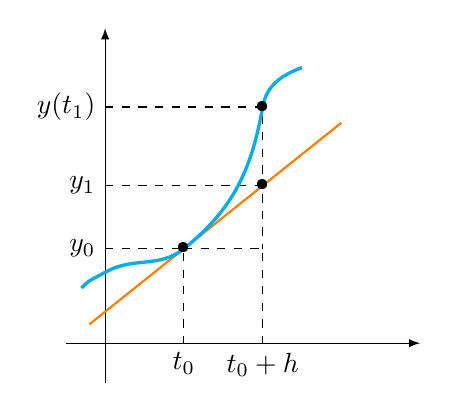
\begin{tikzpicture}[x=1cm,y=1cm]\centering
    \draw[-latex] (-0.5,0)--(4,0); % eixo x
    \draw[-latex] (0,-0.5)--(0,4); % eixo y

    \draw[dashed] (0,1.2) node[left] {$y_0$}--(1,1.2)--(1,0) node[below] {$t_0$}; % y0 -- * -- t0
    \draw[dashed] (1,1.2)--(2,1.2)--(2,0) node[below] {$t_0+h$}; % * -- * -- t_1 = t0+h
    \draw[dashed] (0,2) node[left] {$y_1$}--(2,2)--(2,1.2); % y1 -- * -- t_1 = t0+h
    \draw[dashed] (0,3) node[left] {$y(t_1)$}--(2,3)--(2,2); % y(t1) -- * -- *

    % reta passando pelos pontos (t0, y0) e (t0+h,y1)
    \draw[thick, orange] (-0.2,0.24) -- (3,2.8);

    % a curva
    \draw[very thick, cyan] (-0.3,0.7) 
    to[out=50,in=210] (0,0.9) 
    to[out=30,in=218.66] (1,1.2) 
    to[out=38.66,in=260] (2,3)
    to[out=80,in=200] (2.5,3.5);

    % pontos pretos (bullet)
    \foreach \Point in {(1,1.2),(2,2),(2,3)}{
        \node at \Point {\textbullet};
    }
\end{tikzpicture}
    \caption{Visualização geométrica do método de Euler explícito, onde a curva é a solução exata e a reta é a solução aproximada.}
    \label{fig:euler_explicito_grafico}
\end{figure}

O método de Euler explícito é assim chamado pois fornece explicitamente a sua aproximação em função do instante e do passo anterior, como pode ser visualizado na figura \ref{fig:euler_explicito_grafico}. Uma outra forma de utilizar a primeira derivada é de maneira implícita, no que é chamado \textit{método de Euler implícito}.

\begin{method}[Euler implícito]\label{metodo:euler_implicito}
    Para $h=(b-a)/m$ e $k = 0, 1, ..., m-1$, temos a aproximação:
    \begin{equation*}
        t_{k+1} = t_k + h, \quad
        y_{k+1} = y_k + h f (t_{k+1}, y_{k+1}) = \Phi_h(t_{k+1}, y_{k+1}).
    \end{equation*}
\end{method}

Nesse caso, para avançar a solução no tempo é necessário não apenas aplicar uma fórmula, mas resolver um sistema algébrico de equações geralmente não-lineares no qual $y_{k+1}$ é a incógnita, o que não só exige mais processamento quando utilizado na prática como também pode acumular erros que estão além do método utilizado. Por exemplo, nesses casos é comum utilizar algum método de ponto fixo ou mesmo métodos de Newton ou Quasi-Newton, sendo que nos últimos casos é necessária a estimativa numérica de uma matriz jacobiana $n \times n$ e um certo número de iterações para garantir convergência, o que é custoso e, como todo método numérico, agrega com mais um erro acumulado. Por conta de tudo isso, os métodos numéricos implícitos não foram utilizados nas maiores simulações e não serão tratados neste trabalho. Ainda assim, tais métodos contam com certas vantagens que serão comentadas no decorrer do texto. Mais detalhes dos métodos implícitos e seu uso podem ser encontrados em \cite{Hairer2006-oz}.

Quanto à consistência e à convergência, os métodos propostos são consistentes com 1ª ordem de convergência, pois
\begin{align*}
    e_h(t_{k+1}) 
    &= y(t_{k+1}) - \Phi_h(t_k, \vet y(t_k)) \\
    &= \left(y(t_k) + h \dvet y(t_k) + \dfrac{h^2}{2!} \ddvet y(\xi)\right) - \left( \vet y(t_k) + h f(t_k, \vet y_k) \right) \\
    & = \dfrac{h^2}{2} \ddvet y(\xi),
    \quad
    \xi \in (t_k, t_{k+1}),
\end{align*}
o que pela definição \ref{def:convergencia} implica a ordem 1.

Para exemplificar, considere o problema-modelo \ref{probmodelo:lemniscata} aplicado nos métodos descritos com tamanhos de passo $1/20$, $1/40$, ..., $1/1280$. O resultado pode ser visualizado na tabela \ref{tab:euler_exp_imp_lemniscata}.

\begin{table}[]
    \centering
    \begin{tabular}{c|cc}
        $h$      & Explícito & Implícito   \\
        \hline
        $1/40$   & $0.712071$ & $1.859924$ \\
        $1/80$   & $0.827102$ & $1.283719$ \\
        $1/160$  & $0.904085$ & $1.122329$ \\
        $1/320$  & $0.949289$ & $1.057240$ \\
        $1/640$  & $0.973898$ & $1.027730$ \\
    \end{tabular}
    \caption{Convergência dos métodos de Euler explícito e implícito no problema-modelo \ref{probmodelo:lemniscata}.}
    \label{tab:euler_exp_imp_lemniscata}
\end{table}

Para a aplicação do método de Euler implícito foi utilizado o método de ponto fixo
\begin{equation*}
    \vet y_{k+1}^{[0]} = \vet y_k, \quad \vet y_{k+1}^{[i+1]} = \vet y_k + h f(t_{k+1}, \vet y_{k+1}^{[i]}),
\end{equation*}
para $i=1,...,Q$. Existem diversos critérios para a aplicação deste método \citep[325-335]{Hairer2006-oz}. Porém, como o método não foi de fato utilizado em mais nenhuma outra situação e não foi de nosso interesse neste momento trabalhar com os métodos implícitos no geral, $Q$ foi fixado para $Q=100$ e isso foi mais que suficiente para convergência.


%%%%%%%%%%%%%%%%%%%%%%%%%%%%%%%%%%%%%%%%%%%%%%%%%%%%%%%%%%%%%%%%%
% > METODOS DE RUNGE-KUTTA
%%%%%%%%%%%%%%%%%%%%%%%%%%%%%%%%%%%%%%%%%%%%%%%%%%%%%%%%%%%%%%%%%
\subsection{Métodos de Runge-Kutta}
Uma primeira ideia para obter métodos de ordem mais alta pode ser utilizar séries de Taylor, uma vez que o próprio método de Euler explícito pode ser encontrado via Taylor. O método resultante é como segue.

\begin{method}[Série de Taylor]\label{metodo:taylor}
    Suponha que $f$ do problema \ref{eq:problema_de_cauchy} é de ordem no mínimo $\continuo^q$, e seja $h$ um tamanho de passo fixo. Então
    \begin{equation*}
        \vet \Phi_h(t, \vet y) = y_k + h f(t, \vet y) + \dfrac{h^2}{2!} Df(y,\vet y) + \dfrac{h^3}{3!} D^2 f(t,\vet y) + \hdots + \dfrac{h^q}{q!} D^{q-1} f(t, \vet y),
    \end{equation*}
    onde $D = \derpar{}{t} + f \derpar{}{\vet y}$.
\end{method}

É possível verificar que tal método tem ordem $q$ \citep[42]{alexandre_megiorin_roma_metodos_nodate}. No entanto, tal método traz uma barreira no geral intransponível de maneira analítica para problemas práticos: é preciso encontrar as $q-1$ derivadas de $f$.

Os métodos de Runge-Kutta surgem nesse contexto, a partir da generalização do método de Euler para ordens mais altas, permitindo obter um método de passo único explícito, que concorda com o método \ref{metodo:taylor} para uma dada ordem $q$ e que substitui o cálculo das derivadas de $f$ por médias ponderadas e aplicações de $f$, ou \textit{estágios}, em pontos estratégicos.

\begin{method}[Runge-Kutta de $R$-estágios]\label{metodo:rk_r_estagios}
    Considere o problema \ref{eq:problema_de_cauchy} e tome um tamanho de passo $h$ fixo. Temos
    \begin{equation*}
        \Phi_h(t_k, \vet y_k) = \vet y_k + h \sum_{r=1}^{R} b_r \vet \kappa_r = \vet y_k + h \vet b^T \bm K,
        \quad \bm K = (\kappa_1, ..., \kappa_R)
    \end{equation*}
    onde
    \begin{align*}
        \vet \kappa_r (t,\vet y) &= f\left(t + h c_r, \vet y + h \sum_{j=1}^R a_{rj} \vet \kappa_j \right),
        \quad 1 \leq r \leq R.
    \end{align*}
\end{method}

Os parâmetros $a_{rj}$, $b_r$ e $c_r$ variam para cada método, mas para métodos explícitos sempre satisfazem as relações
\begin{equation}\label{eq:hipoteses_runge_kutta_explicito}
    \begin{aligned}
        \text{(i)} \quad & \sum_{r=1}^{R} b_r = 1, \\
        \text{(ii)} \quad & c_r = \sum_{j=1}^{r-1} a_{rj}, \quad 2 \leq r \leq R.
    \end{aligned}
\end{equation}

A condição (i) é suficiente e necessária para consistência, pois $h \to 0$ leva $\vet \kappa_r (t, \vet y) \to f (t, \vet y)$, então
\begin{equation*}
    \sum_{r=1}^{R} b_r \vet \kappa_r  = f(t,y) \sum_{r=1}^R b_r = f(t,\vet y).
\end{equation*}
Já (ii) garante a concordância com o método de Taylor, conforme \cite[45]{alexandre_megiorin_roma_metodos_nodate}.

Uma notação comum para representar as constantes $a_{rj}$, $b_r$ e $c_r$ é a Tabela de Butcher, dada pela seguinte forma:
\begin{table}
    \centering
    \begin{tabular}{c|c}
         $\vet c$ & $\bm A$\\
         \hline
                  & $\vet b$
    \end{tabular}
    \caption{Tabela de Butcher.}
\end{table}

Observe que o método de Euler explícito (método \ref{metodo:euler_explicito}) é um método de Runge-Kutta de ordem 1 com tabela
\begin{table}
    \centering
    \begin{tabular}{c|ccccc}
         $0$      & \\
         \hline
                  & 1
    \end{tabular}
    \quad
    \begin{tabular}{c|ccccc}
         $1$      & 1  \\
         \hline
                  & 1
    \end{tabular}
    \caption{Tabela de Butcher para os métodos de Euler explícito e implícito, respectivamente.}
\end{table}

Uma grande quantidade de métodos de Runge-Kutta é conhecida, com as mais diferentes ordens. Vale ressaltar também que a ordem de um método de Runge-Kutta é sempre menor ou igual ao número de estágios, ou seja, um método explícito de ordem $p$ tem uma quantidade de estágios $s \geq p$. Mais ainda, se $p \geq 5$, então $s > p$. No geral, parece existir uma tendência de que conforme $p$ aumenta, o valor mínimo de $s$ passa a ser $p + k_p$, para $k_p$ uma constante associada a $p$. Isso, porém, é ainda um problema não resolvido acerca dos métodos de Runge-Kutta \citep[187-196]{Butcher2016-jx}.

Apresentamos a seguir os métodos de ordem 2, 3 e 4, que são os métodos tradicionais mais frequentemente utilizados \citep[46-47]{alexandre_megiorin_roma_metodos_nodate}.

\begin{method}[Runge-Kutta de Segunda Ordem e Dois Estágios (RK22)]\label{metodo:rk22} 
    O método RK22 tem a seguinte Tabela de Butcher:
    \begin{table}[H]
        \centering
        \begin{tabular}{c|cccc}
             $0$      &       &      \\
             $1/2$    & $1/2$  &      \\
             \hline
                      & $0$ & $1$
        \end{tabular}
        \caption{Tabela de Butcher para o método RK22.}
    \end{table}
\end{method}

\begin{method}[Runge-Kutta de Terceira Ordem e Três Estágios (RK33)]\label{metodo:rk33} 
    O método RK33 tem a seguinte Tabela de Butcher:
    \begin{table}[H]
        \centering
        \begin{tabular}{c|cccc}
             $0$      &       &       &     \\
             $1/2$    & $1/2$ &       &     \\
             $1$      & $-1$   & $2$  &     \\
             \hline
                      & $1/6$ & $4/6$ & $1/6$
        \end{tabular}
        \caption{Tabela de Butcher para o método RK33.}
    \end{table}
\end{method}

\begin{method}[Runge-Kutta de Quarta Ordem e Quatro Estágios (RK44)]\label{metodo:rk44} 
    O método RK44 tem a seguinte Tabela de Butcher:
    \begin{table}[H]
        \centering
        \begin{tabular}{c|ccccc}
             $0$      &       &       &       &\\
             $1/2$    & $1/2$ &       &       &\\
             $1/2$    & $0$   & $1/2$ &       &\\
             $1$      & $0$   & $0$   & $1$   & \\
             \hline
                      & $1/6$ & $1/3$ & $1/3$ & $1/6$
        \end{tabular}
        \caption{Tabela de Butcher para o método RK44.}
    \end{table}
\end{method}

O mesmo método para depuração da ordem dos métodos (ver (\ref{eq:aproximacao_ordem})) pode ser aplicado para os métodos de Runge-Kutta no problema-modelo \ref{probmodelo:lemniscata}. O resultado consta na tabela \ref{tab:rk_lemniscata}.

\begin{table}[]
    \centering
    \begin{tabular}{c|ccc}
        $h$     & RK22 & RK33 & RK44 \\
        \hline
        $1/40$  & $1.989241$ & $2.936490$ & $4.041771$ \\
        $1/80$  & $2.003212$ & $2.965188$ & $4.025951$ \\
        $1/160$ & $2.003873$ & $2.981701$ & $4.014280$ \\
        $1/320$ & $2.002516$ & $2.990612$ & $4.008214$ \\
        $1/640$ & $2.001404$ & $2.995243$ & $3.992159$ \\
    \end{tabular}
    \caption{Convergência dos métodos RK22, RK33 e RK44 no problema-modelo \ref{probmodelo:lemniscata}}
    \label{tab:rk_lemniscata}
\end{table}


%%%%%%%%%%%%%%%%%%%%%%%%%%%%%%%%%%%%%%%%%%%%%%%%%%%%%%%%%%%%%%%%%
% > ESTABILIDADE DOS METODOS TRADICIONAIS
%%%%%%%%%%%%%%%%%%%%%%%%%%%%%%%%%%%%%%%%%%%%%%%%%%%%%%%%%%%%%%%%%
\subsection{Estabilidade dos integradores tradicionais}
Outra questão importante a se analisar sobre integradores numéricos é como se comportam em intervalos ilimitados, não apenas em intervalos limitados como feito até então. Para isso, é utilizado como problema modelo o problema de valor inicial mais simples possível:
\begin{equation}\label{eq:edo_problema_linear}
    \dvet y(t) = \bm M \vet y(t), \quad \vet y(t_0) = \vet y_0,
\end{equation}
sendo $\bm M$ uma matriz constante. O método de Euler explícito aplicado com um tamanho de passo $h$ assume a seguinte forma para o instante $t_k = t_0 + k h$:
\begin{equation}\label{eq:edo_linear_aproximacao}
    \vet y_k = (\bm I + h \bm M) \vet y_{k-1}
    \quad
    \therefore
    \quad
    \vet y_k = (\bm I + h \bm M)^k \vet y_0.   
\end{equation}
Além disso, da teoria de equações diferenciais, sabemos que a solução exata do problema (\ref{eq:edo_problema_linear}) é
\begin{equation}\label{eq:edo_linear_solucao}
    \vet y(t_k) = \exp{(k h \bm M)} \vet y_0.
\end{equation}

Considere uma mudança de base tal que $\vet y(t) = \bm A \vet z(t)$ e $\vet y_k = \bm A \vet z_k$, sendo $\bm A$ uma matriz constante e não singular. Temos então o problema nas novas coordenadas:
\begin{equation}
    \dvet z (t) = \bm A^{-1} \bm M \bm A \vet z(t) = \bm B \vet z(t),
    \quad
    \vet z(t_0) = \vet z_0,
\end{equation}
com solução exata
\begin{equation}
    \vet z(t_k) = \exp{(k h \bm B)} \vet z_0
\end{equation}
e solução aproximada
\begin{equation}
    \vet z_k = (\bm I + h \bm B)^k \vet z_0.
\end{equation}
Se a transformação escolhida é tal que $\bm B$ é a forma canônica de Jordan de $\bm M$, então para cada autovalor $\lambda$ tem-se uma equação diferencial da forma
\begin{equation}
    \dvet y(t) = \lambda \vet y(t),
\end{equation}
chamada \textbf{problema modelo} se $\RePart{\lambda} < 0$, com solução
\begin{equation}
    \vet y(t_k) = \exp{(k h \lambda}) \vet y_0.
\end{equation}
Assim, para o método de Euler explícito ser adequado é necessário que $(1+ h \lambda)^k$ seja uma aproximação aceitável para $\exp{(k h \lambda)}$, ou que no mínimo $(1+h \lambda)^k$ tenha comportamento limitado para $k \to \infty$ quando $\exp{(k h \lambda)}$ for limitado. Isso ocorre se e somente se $|1 + h \lambda| \leq 1$. Tomando $z = h \lambda$, a região complexa $|1+z| \leq 1$ é chamada de \textbf{região estável} para o método de Euler explícito, conforme figura \ref{fig:regiao_estabilidade_euler_explicito}.

\begin{figure}
    \centering
    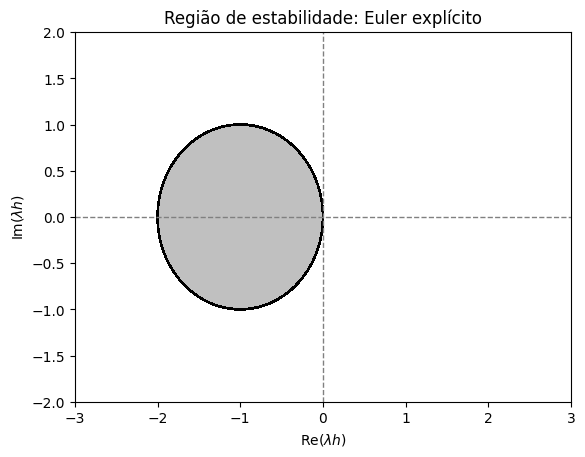
\includegraphics[width=0.5\linewidth]{tcc//img/regiao_estabilidade_euler.png}
    \caption{Região de estabilidade para o método de Euler explícito.}
    \label{fig:regiao_estabilidade_euler_explicito}
\end{figure}

\begin{definition}[Estabilidade de métodos numéricos]
    O problema de valor inicial
    \begin{equation*}
        \dot y(t) = \lambda y(t),
        \quad
        y(t_0) = y_0,
        \quad \RePart{\lambda} < 0
    \end{equation*}
    é chamado de \textbf{problema modelo}. Considere um método de passo único que aplicado ao problema modelo fornece a expressão
    \begin{equation*}
        y_{k+1} = \phi (\lambda h) y_k.
    \end{equation*}
    O conjunto $\Omega = \{\eta \in \mathbb{C} : |\phi(\eta)| < 1 \}$ é denominado \textbf{região de estabilidade absoluta} para $h>0$ fixado, $\phi(\lambda h)$ é chamado \textbf{fator de amplificação} e o intervalo $I_e = \Omega \cap \R$ é o \textbf{intervalo de estabilidade absoluta} do método. Um método \textbf{absolutamente estável} é também chamado de \textbf{A-estável}.
\end{definition}

Observando a região de estabilidade do método de Euler explícito, é fácil concluir que o método não é A-estável, uma vez que $|1+h \lambda| \leq 1$ somente se $h \leq - \RePart{\lambda} / |\lambda|$. Dizemos então que trata-se de um método \textbf{condicionalmente estável}.

Por outro lado, o método de Euler implícito (método \ref{metodo:euler_implicito}) tem uma comportamento diferente. Aplicando o mesmo processo anterior, obtemos a expressão
\begin{equation}
    \vet y_k = (1 - z)^{-1} \vet y_{k-1},
\end{equation}
e então sua região estável é $|1-z| \geq 1$, como na figura \ref{fig:regiao_estabilidade_euler_implicito}. Nesse caso, $\phi (\lambda h) = (1 - \lambda h)^{-1}$, então para qualquer $h > 0$ temos que $|\phi(\lambda h)| < 1$.

\begin{figure}
    \centering
    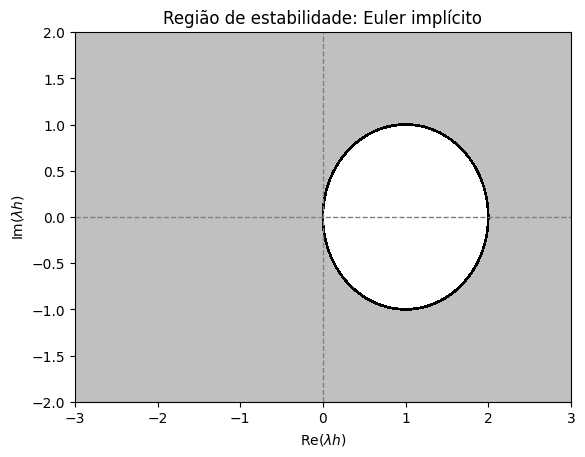
\includegraphics[width=0.5\linewidth]{tcc/img/regiao_estabilidade_euler_implicito.png}
    \caption{Região de estabilidade do método de Euler implícito}
    \label{fig:regiao_estabilidade_euler_implicito}
\end{figure}

É possível generalizar essa ideia para os métodos de Runge-Kutta. Tomando um método de ordem $s$ com tabela
\begin{table}
    \centering
    \begin{tabular}{c|c}
        $\vet c$ &  $\bm A$ \\
        \hline & $\vet b^T$
    \end{tabular}
\end{table}\\
temos para o problema modelo:
\begin{equation}
    \bm K = (\bm I - h \lambda \bm A)^{-1} \lambda \bm 1 y_0
    = (\bm I - z \bm A)^{-1} \lambda \bm 1 y_0,
\end{equation}
então
\begin{equation}\label{eq:ampliacao_rk_geral}
    y_1 
    = y_0 + h \vet b^T \bm K
    = [1 + z \vet b^T (\bm I - z \bm A)^{-1} \bm 1] y_0
    = R(z) y_0,
\end{equation}
sendo $R(\vet z)$ o fator de ampliação do método. Para o caso de métodos explícitos, a matriz $\bm A$ é triangular com diagonal nula, e portanto nilpotente com algum grau $k$. Através de uma expansão algébrica pode-se concluir que
\begin{equation}\label{eq:inversa_nilpotentes}
    (\bm I - z \bm A) = \bm I + \sum_{j=1}^{k-1} z^j \bm A^k.
\end{equation}
Substituindo (\ref{eq:inversa_nilpotentes}) em (\ref{eq:ampliacao_rk_geral}),
\begin{align*}
    R(z) 
    &= 1 + z \vet b^T (\bm I + \sum_{j=1}^{k-1} z^j \bm A^j)\bm 1 \\
    &= 1 + z \vet b^T \bm I \bm 1 + \vet b^T \sum_{j=1}^{k-1} z^{j+1} \bm A^j \bm 1.
\end{align*}
A partir de (\ref{eq:hipoteses_runge_kutta_explicito}), temos por (i) que $\vet b^T \bm I \bm 1 = \sum_{j=1}^s b_j = 1$. Temos então que
\begin{equation}
    R(z) = 1 + z + \sum_{j=1}^{k-1} z^{j+1} \bm A^j \bm 1.
\end{equation}
No caso dos métodos explícitos em que $p=s$, temos os seguintes fatores:
\begin{equation}
    R (z) = \begin{cases}
    1 + z, & p = 1, \\
    1 + z + \frac{1}{2} z^2, & p = 2, \\
    1 + z + \frac{1}{2} z^2 + \frac{1}{6} z^3, & p = 3, \\
    1 + z + \frac{1}{2} z^2 + \frac{1}{6} z^3 + \frac{1}{24} z^4, & p = 4.
    \end{cases}
\end{equation}
A região de estabilidade absoluta desses métodos pode ser vista na figura \ref{fig:regiao_estabilidade_rk_explicitos}, sendo o interior de cada curva fechada.

\begin{figure}
    \centering
    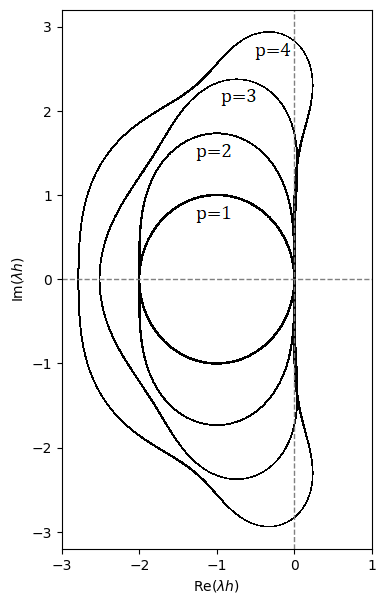
\includegraphics[width=0.35\linewidth]{tcc//img/regiao_estabilidade_rk.png}
    \caption{Região de estabilidade dos métodos de Runge-Kutta de ordens e estágios $p = 1, 2, 3$ e $4$.}
    \label{fig:regiao_estabilidade_rk_explicitos}
\end{figure}

Uma vez que as regiões de estabilidade são fechadas pois o fator é polinomial, os métodos de Runge-Kutta explícitos não são A-estáveis. Porém, da mesma forma que no caso dos métodos de Euler explícito e implícito, é possível obter A-estabilidade utilizando métodos implícitos. 
\begin{table}[H]
    \centering

    \begin{tabular}{c|cc}
        $\frac{1}{2} - \frac{\sqrt 3}{6}$ & $1/4$ & $\frac{1}{4} - \frac{\sqrt 3}{6}$ \\
        $\frac{1}{2} + \frac{\sqrt 3}{6}$ & $\frac{1}{4} + \frac{\sqrt 3}{6}$ & $1/4$ \\
        \hline & $1/2$ & $1/2$
    \end{tabular}
    
    \caption{Método de Runge-Kutta implícito de quarta ordem e dois estágios. \citep[99]{Butcher2016-jx}}.
    \label{tab:exemplo_metodo_runge_kutta_implicito}
\end{table}

Por exemplo, considere o método de quarta ordem da tabela \ref{tab:exemplo_metodo_runge_kutta_implicito}. Seu fator de amplificação é
\begin{equation*}
    R(z) = \dfrac{1 + \frac{z}{2} + \frac{z^2}{12}}{1 - \frac{z}{2} + \frac{z^2}{12}}.
\end{equation*}
Observe que $|R(z)| \leq 1$ somente se $\RePart{z} \leq 0$, e uma vez que $z = \lambda h$ com $\RePart{\lambda} < 0$, qualquer valor de $h$ garante estabilidade para o método, sendo então A-estável.

Apesar da maior facilidade para obter métodos implícitos de altas ordens e estáveis, a necessidade de utilizar métodos iterativos para resolver o sistema de equações pode não compensar computacionalmente tais ganhos qualitativos. Ainda assim, os métodos de Runge-Kutta implícitos são utilizados em diversas aplicações, inclusive porque todas as versões simpléticas dos métodos RK são necessariamente implícitas (veja o Teorema \ref{teorema:rk_simpletico}).

De toda forma, a A-estabilidade, por definição, se aplica para problemas lineares, o que não é o caso da grande maioria de aplicações práticas dos integradores numéricos. No entanto, muitos sistemas podem ser aproximados localmente por sua linearização, sendo então possível aplicar os resultados de estabilidade para obter tamanhos de passo adequados.

No problema de N-corpos, utilizar o método de Euler implícito não apresentou nenhuma vantagem. No entanto, ainda é possível observar algumas anomalias esperadas para cada método simulando, por exemplo, o problema-modelo \ref{probmodelo:lemniscata}. Na figura \ref{fig:lemniscata_euler_exp_imp_distancia} é possível observar a diferença na divergência entre os dois métodos quando comparados a um método simplético de alta ordem. Enquanto o método de Euler explícito apresenta um afastamento de órbita mais prolongado, o método de Euler implícito apresenta afastamentos mais breves.

\begin{figure}
    \centering
    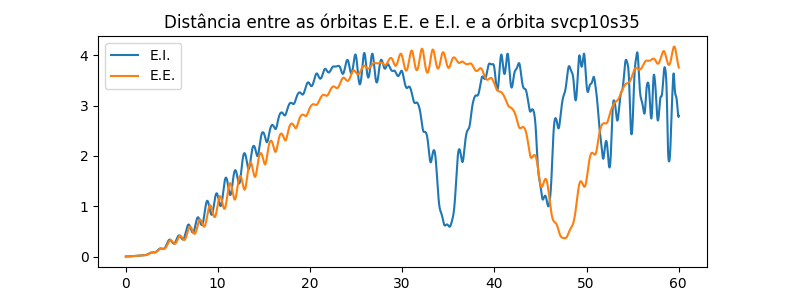
\includegraphics[width=0.75\linewidth]{tcc//img/lemniscata_euler_exp_imp_svcp10s35.png}
    \caption{Distância no espaço de fases entre as soluções numéricas do problema-modelo \ref{probmodelo:lemniscata} com métodos de Euler explícito e implícito e o método svcp10s35 com $h=10^{-3}$ no intervalo $[0,60]$.}
    \label{fig:lemniscata_euler_exp_imp_distancia}
\end{figure}

Um motivo para isso pode ser observado na figura \ref{fig:lemniscata_euler_exp_imp}. Uma vez que $E_0 - E$ decresce no método de Euler explícito, a energia total está aumentando, o que significa que a energia cinética está aumentando (ou que a potencial está diminuindo). Isso leva a um relaxamento do período e com aproximações mais violentas, e portanto ao menos uma partícula deve ser ejetada do sistema em sua evolução.

Já no caso implícito, $E_0-E$ cresce, logo a energia total está diminuindo, então a energia potencial está aumentando (ou a energia cinética está diminuindo). Isso implica no encolhimento do período, e como o PNCG pode conter colisões o sistema fica numericamente instável.

Na prática, o método de Euler explícito ``erra para mais'', expandindo a trajetória, enquanto o método de Euler implícito ``erra para menos'', contraindo a trajetória.

\begin{figure}
        \centering
        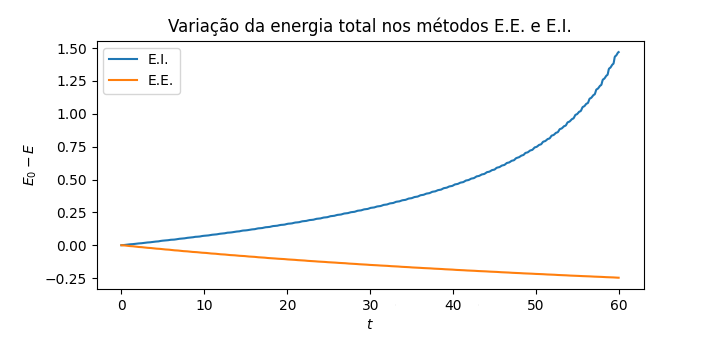
\includegraphics[width=0.7\linewidth]{tcc//img/lemniscata_euler_exp_imp.png}
        \caption{Variação (com sinal) da energia total em simulações do problema-modelo \ref{probmodelo:lemniscata} via métodos de Euler explícito e implícito e com $h=10^{-3}$ no intervalo $[0,60]$.}
        \label{fig:lemniscata_euler_exp_imp}
\end{figure}